% Created 2024-12-18 Wed 14:05
% Intended LaTeX compiler: pdflatex
\documentclass[10pt]{article}
% =================================BASE====================================%
\usepackage[left=2cm,right=2cm,top=2cm,bottom=2cm]{geometry} % Marges
\usepackage[T1]{fontenc} % Nécessaire avec FrenchBabel
\usepackage[utf8]{inputenc} % Important pour symboles Francophones, é,à,etc
\usepackage{csquotes} % Recommandé par PDFLatex lors de la compilation. 

% Calligraphie
%\usepackage{pxfonts} % Met le texte ET les maths en Palatino + donne accès à des symboles math
%\usepackage{palatino} % Cette commande met seulement le texte en police palatino
\usepackage{lmodern} % Pour les maths? Lmodern pour les maths
\usepackage{cfr-lm} % Use lmodern for sans-serif
\usepackage{mathrsfs} % Permet la command \mathscr (Lettres attachées genre) \mathscr(ABC)
\usepackage{eucal}   % Vient changer le \mathcal{ABC} parce que celui de base est laid.

% Bibliographie
\usepackage[backend=biber,sorting=ynt,maxbibnames=99,style=authoryear]{biblatex}
\addbibresource{master-bibliography.bib}

% Stuff
\usepackage{amsmath, amssymb, amsthm} % Symb. math. (Mathmode+Textmode) + Beaux théorèmes.
\usepackage{mathtools,cancel,xfrac} % Utilisation de boîtes \boxed{} + \cancelto{}{}, xfrac
\usepackage{graphicx, wrapfig} % Géstion des figures.
\usepackage{hyperref} % Permettre l'utilisation d'hyperliens.
\usepackage{color} % Permettre l'utilisation des couleurs.
\usepackage{colortbl} % Color tables
\usepackage[dvipsnames]{xcolor} % Couleurs avancées.

% Physique
\usepackage{physics} % Meilleur package pour physicien. 

% Style
\usepackage{pgf,tikz} % Realisation de figures TIKZ.
\usetikzlibrary{arrows.meta,bending, shapes.geometric, automata, positioning, decorations.pathreplacing, math} % Arrow heads et les formes de noeuds
\usepackage{empheq} % Boite autour de MULTIPLE équations
\usepackage{bbding}

% Français
\usepackage[french]{babel} % Environnements en Français.
\frenchbsetup{
StandardLists=true,
StandardItemLabels=true} % Sinon, french modifie les itemize
\usepackage{titling} % Donne accès à \theauthor, \thetitle, \thedate
% ==============================BASE-(END)=================================%





% ================================SETTINGS=================================%
% Pas d'indentation en début de paragraphe :
\setlength\parindent{0pt}
\setlength{\parskip}{0.15cm}

% Tableaux/tabular
% Espace vertical dans les tabular/tableaux
\renewcommand{\arraystretch}{1.2}

% Couleurs de hyperliens :
\definecolor{mypink}{RGB}{147, 0, 255}
\hypersetup{colorlinks, 
             filecolor=mypink,
             urlcolor=mypink, 
             citecolor=mypink, 
             linkcolor=mypink, 
             anchorcolor=mypink}
\definecolor{color1}{RGB}{148,220,236}
\definecolor{color2}{RGB}{84,76,163}
\definecolor{color3}{RGB}{108,156,227}
\definecolor{color4}{RGB}{244,164,156}
\definecolor{color5}{RGB}{252,204,164}


% Numéros d'équations suivent les sections :
\numberwithin{equation}{section} 


% Les « captions » sont en italique et largeur limitée
\usepackage[textfont = it]{caption} 
\captionsetup[wrapfigure]{margin=0.5cm}


% Retirer l'écriture en gras dans la table des matières
\usepackage{tocloft}
\renewcommand{\cftsecfont}{\normalfont}
\renewcommand{\cftsecpagefont}{\normalfont}


% MODIFICATION DES TITLESECS et SUBTITLESEC
% On a des lignes à droite des sections et sous-sections
\usepackage[explicit]{titlesec}
    % Raised Rule Command:
    % Arg 1 (Optional) - How high to raise the rule
    % Arg 2 - Thickness of the rule
    \newcommand{\raisedrulefill}[2][0ex]{\leaders\hbox{\rule[#1]{1pt}{#2}}\hfill}
    \titleformat{\section}{\Large\bfseries}{\thesection. }{0em}{#1\;\raisedrulefill[0.4ex]{0.25pt}}
    \titleformat{\subsection}{\large\bfseries}{\thesubsection. }{0em}{#1\;\raisedrulefill[0.4ex]{0.10pt}}


% MODIFICATION DES LISTES : 
\renewcommand{\labelitemi  }{{\raisebox{0.35\height}{\tiny$\blacksquare$}}}
\renewcommand{\labelitemii }{{\raisebox{0.35\height}{\tiny$\blacktriangleright$}}}
\renewcommand{\labelitemiii}{$\bullet$}

\renewcommand{\boxtimes}{\blacksquare}
% ================================SETTINGS=================================%



% ==============================NEWCOMMANDS================================%
% CQFD symbol
\renewcommand{\qedsymbol}{$\hfill\blacksquare$}
\newcommand{\cqfd}{\hfill$\blacktriangleleft$}

% Vecteurs de base :
\newcommand{\nvf}{\vb{\hat{n}}}
\newcommand{\evf}{\vb{\hat{e}}}
\newcommand{\ivf}{\vb{\hat{i}}}
\newcommand{\jvf}{\vb{\hat{j}}}
\newcommand{\kvf}{\vb{\hat{k}}}
\newcommand{\uu}{\vb{u}}
\newcommand{\vv}{\vb{v}}
\newcommand{\ust}{\vb{u}_{\ast}}
\newcommand{\xx}{\vb{x}}
\newcommand{\rad}{\text{Rad}}

% Physics empty spaces 
\newcommand{\short}{\vphantom{pA}}
\newcommand{\tall}{\vphantom{pA^{x^x}_p}}
\newcommand{\grande}{\vphantom{\frac{1}{xx}}}
\newcommand{\venti}{\vphantom{\sum_x^x}}
\newcommand{\pt}{\hspace{1pt}} % One horizontal pt space

% Moyenne numérique entre deux points de grilles. 
\newcommand{\xmean}[1]{\overline{#1}^x}
\newcommand{\ymean}[1]{\overline{#1}^y}
\newcommand{\zmean}[1]{\overline{#1}^z}
\newcommand{\xymean}[1]{\overline{#1}^{xy}}

% Tilde over psi
\newcommand{\tpsi}{\tilde{\psi}}
\newcommand{\tphi}{\tilde{\phi}}

% Nota Bene env :
%\newcommand{\nb}{$\boxed{\text{\footnotesize\EightStarConvex}\pt \mathfrak{N. B.}}$\hspace{4pt}}
\newcommand{\nb}{\underline{{\footnotesize\EightStarConvex}\pt $\mathfrak{N.B.}$\vphantom{p}}\hspace{3pt}}

% Opérateur de transformée de Fourier. 
\newcommand{\fourier}{\operatorname{\raisebox{-0.4em}{\resizebox{2em}{!}{$\mathscr{F}$}}}}

% Mettre (a,b) à la suite d'une série d'équations horizontales.
\newcommand{\ab}{\refstepcounter{equation}\tag{\theequation a,b}}
% ==============================NEWCOMMANDS================================%



% ==============================PAGE-TITRE=================================%
% Titlepage 
\newcommand{\mytitlepage}{
\begin{titlepage}
\begin{center}
{\Huge \thesubtitle \par}
\vspace{2cm}
{\Huge \MakeUppercase{\thetitle} \par}
\vspace{2cm}
RÉALISÉ DANS LE CADRE\\ D'UN PROJET POUR \par
\vspace{2cm}
{\Huge ISMER--UQAR \par}
\vspace{2cm}
{\thedate}
\end{center}
\vfill
Rédaction \\
{\theauthor}\\
\url{charles-edouard.lizotte@uqar.ca}\\
ISMER-UQAR\\
Police d'écriture : \textbf{CMU Serif Roman}
\end{titlepage}
}
% ==============================PAGE-TITRE=================================%



% =================================ENTÊTE==================================%
\usepackage{fancyhdr}
\pagestyle{fancy}
\setlength{\headheight}{13pt}
\renewcommand{\headrulewidth}{0.0pt} % Ligne horizontale en haut

\fancyhead[R]{\underline{\textit{Section \thesubsection}}}
\fancyhead[L]{\underline{\textit{\thepage}}}
\fancyfoot[R]{\textit{\theauthor}}
\fancyfoot[L]{}
\fancyfoot[C]{} 
% =================================ENTÊTE==================================%
\author{Charles-Édouard Lizotte}
\date{15/11/2024}
\title{Rapport hebdomadaire}
\newcommand{\thesubtitle}{Contrat Été 2024}
\hypersetup{
 pdfauthor={Charles-Édouard Lizotte},
 pdftitle={Rapport hebdomadaire},
 pdfkeywords={},
 pdfsubject={},
 pdfcreator={Emacs 29.4 (Org mode 9.7.11)}, 
 pdflang={French}}
\begin{document}

\mytitlepage
\tableofcontents\newpage
\section{Rencontre avec Dany}
\label{sec:org542a210}

\begin{itemize}
\item Le cas que nous avions créé dans le but d'immiter les expériences d'Eliot Bismuth ne couvraient qu'un seul point de grille avec un bon nombre (10) de points sous-grille. Il faut drait plutôt plusieurs points de grille avec un nombre plus grand de points de grilles, selon Dany.

\item Le cas sans glace n'a aucune valeur selon Dany. En outre, dans le cas sans glace, la \emph{spectral tail} prend une trop grande ampleur et l'on perd un peu. Ce cas n'est seulement important que pour comparer l'effet de la résolution sur le modèle de vagues.

\item Encore une fois, il faudrait bien poser la question, mais la présentation que j'ai fait couvre bien l'enjeu du problème.

\item Il a aussi été mentionné que la taille des points de grille sur les modèle globaux tournent autour de 5 km, donc il faudrait mettre un peu d'effort là. \newpage
\end{itemize}
\section{Retour sur la méthode}
\label{sec:orgf3f2c9a}

Rapidement, toutes les sous-mailles (lorsqu'on augmente la résolution) sont des multiples de 2, de sorte qu'on peut augmenter la résolution avec la méthode ci-bas : 

\tikzmath{\lx=28;\ly=3;}

\begin{figure}[!h]
\begin{center}
   \begin{tikzpicture}[scale=0.6]
      % Green!25
      \fill [color=Green!25] (0,0) rectangle (\lx,1);
      \fill [color=Green!25] (0,2) rectangle (\lx,3);
      \fill [color=Aquamarine!75] (8,1) rectangle (\lx-4,2);
      \fill [BrickRed!35] (4,1) rectangle (8,2);
      \fill [Dandelion!35] (0,1) rectangle (4,2);
      \fill [Dandelion!35] (24,1) rectangle (28,2);
      \foreach \y in {0,...,\ly} {
         \draw [ultra thick, white] (0,\y) -- (\lx,\y);
         \foreach \x in {0,4,...,\lx} {
            \draw [ultra thick, white] (\x,0) -- (\x,3);
            }
         }
      \draw [black, ultra thin] (0,0) rectangle (\lx,\ly);
      \draw [black,|{latex}-{latex}|] (0,3.5) -- (28,3.5);
      \draw (14,3.5) node [above] {$L_x$};
      \draw (26,1.5) node [] {$nx=7$};
   \end{tikzpicture}\medskip
   
   \begin{tikzpicture}[scale=0.6]
      \fill [color=Green!25] (0,0) rectangle (\lx,1);
      \fill [color=Green!25] (0,2) rectangle (\lx,3);
      \fill [color=Aquamarine!75] (8,1) rectangle (\lx-4,2);
      \fill [BrickRed!35] (2,1) rectangle (8,2);
      \fill [Dandelion!35] (24,1) rectangle (28,2);
      \fill [Dandelion!35] (0,1) rectangle (6,2);
      \foreach \y in {0,...,\ly} {
         \draw [ultra thick, white] (0,\y) -- (\lx,\y);
         \foreach \x in {0,2,...,\lx} {
            \draw [ultra thick, white] (\x,0) -- (\x,3);
            }
         }
      \draw [black, ultra thin] (0,0) rectangle (\lx,\ly);
      \draw (26,1.5) node [] {$nx=14$};
   \end{tikzpicture}\medskip
   
   \begin{tikzpicture}[scale=0.6]
      \fill [color=Green!25] (0,0) rectangle (\lx,1);
      \fill [color=Green!25] (0,2) rectangle (\lx,3);
      \fill [color=Aquamarine!75] (8,1) rectangle (\lx-4,2);
      \fill [BrickRed!35] (3,1) rectangle (8,2);
      \fill [Dandelion!35] (24,1) rectangle (28,2);
      \fill [Dandelion!35] (0,1) rectangle (7,2);
      \foreach \y in {0,...,\ly} {
         \draw [ultra thick, white] (0,\y) -- (\lx,\y);
         \foreach \x in {0,1,...,\lx} {
            \draw [ultra thick, white] (\x,0) -- (\x,3);
            }
         }
      \draw [black, ultra thin] (0,0) rectangle (\lx,\ly);
      \draw [black,|{latex}-{latex}|] (8,-1) -- (16.5,-1) node [fill=white] {$n_{x,m} = (n_0-3)\times2^k = 4\times 2^n$} -- (24,-1);
      \draw (26,1.5) node [] {$nx=28$};
   \end{tikzpicture}
   \begin{minipage}{0.8\linewidth}
      \caption{Schéma conceptuelle de la carte d'allocation des sous-mailles lorsqu'on augmente la résolution.}
   \end{minipage}
\end{center}
\end{figure}

\begin{itemize}
\item Pourquoi cette forme étrange? Selon la documentation de \emph{wavewatch},
\end{itemize}
\begin{quote}
« \emph{Outer grid lines are always defined as land points} »
\end{quote}
Et tous les paramètres de l'expériences sont tabulés dans le tableau ci-dessous : 

\begin{center}
\begin{tabular}{cllc}
\hline
\hline
Variables & Description & Valeur & Unités\\
\hline
\(n_{x,0}\) & Nombre initial de points & 11 & --\\
\(n_{x.m}\) & Nombre de points de mer (\emph{inner nx}) & \{8,16,32,64\} & \\
\(kx\) & Multiplicateur de 2 & \{0,1,2,\ldots{}\} & --\\
\(sdfx\) & \emph{Scaling (divison) factor} (\(2^k\)) & \{1,2,4,\ldots{}\} & --\\
\(n_x\) & Nombre de points de grille & \(n_{x,0}\times2^k\) & --\\
\(\max(n_x)\) & Nombre de points de grille (haute résolution) & 88 & --\\
\(\min(n_x)\) & Nombre de points de grille (haute résolution) & 11 & --\\
\hline
\(L_x\) & Longueur totale du domaine & 8800 & m\\
\(L_y\) & Largeur totale du domaine & 300 & m\\
\(\Delta x\) & Longueur horizontale des sous-mailles & \{800,100\} & m\\
\(\Delta y\) & Longueur verticale des sous-mailles & 100 & m\\
\hline
\(u_{10}\) & Vent à 10m au dessus de la surface & 10 & ms\textsuperscript{-1}\\
\(u_o\) & Vitesse du courant à la surface & 0 & ms\textsuperscript{-1}\\
\(ice frac\) & Fraction de glace du domaine & \{0,0.25,0.5,0.75\} & --\\
\(f_i\) & Fraction de glace des points de grille & \{0,0.25,0.5,0.75\} & --\\
\hline
\end{tabular}
\end{center}

\begin{itemize}
\item Lorsqu'on fait mention de la \emph{ice fraction}, on parle de
\begin{equation}
   \mathit{ice\, frac} = \expval{f_i} = \frac{1}{n_{x,mer}}\sum_i f_i.
\end{equation}
\end{itemize}
\subsection{Retour sur les conditions frontière}
\label{sec:org435e436}


Tirée de la \href{https://wavespectra.readthedocs.io/en/latest/construction.html\#jonswap}{documentation du module Wavespectra}, le spectre d'énergie du JONSWAP \autocite[voir][]{hasselmann1973measurements} est donnée par
\begin{equation}
\label{eq:org8bfebe5}
   S(f) = \alpha g^2 (2\pi)^{-4} f^{-5} \exp{-\frac{5}{4} \left (\frac{f}{f_p} \right)^{-4} } \gamma^{\exp{\frac{(f-f_p)^2}{2\sigma^2f_p^2}}}.
\end{equation}
Cette version est totalement indépendante de la hauteur significative des vagues, contrairement à la version d'Eliot Bismuth. Par contre, toujours selon la documentation du module Wavespectra, lorsque la hauteur significative des vagues est fournie, le spectre \ref{eq:org8bfebe5} est normalisé de sorte à ce que \(4\sqrt{m_0} = Hs\). Autrement, le spectre est normalisé par \(\alpha\) comme précédemment.\bigskip

Finalement, la fonction de l'étalement directionnel \(G(\theta,f)\) est exprimée par
\begin{equation}
   G(\theta,f)=F(s)cos^2\qty[\frac{1}{2}(\theta-\theta_{m})],
\end{equation}
où \(F(s)\) est seulement un paramètre de normalisation -- car l'intégrale sur le domaine doit être de 1. Le résultat, c'est la figure \ref{fig:jonswap}. Les paramètre des conditions frontière sont tabulés dans le tableau \ref{tab:org361184d}. 

\begin{figure}[!h]
\begin{center}
\begin{minipage}{0.5\textwidth}
\begin{center}
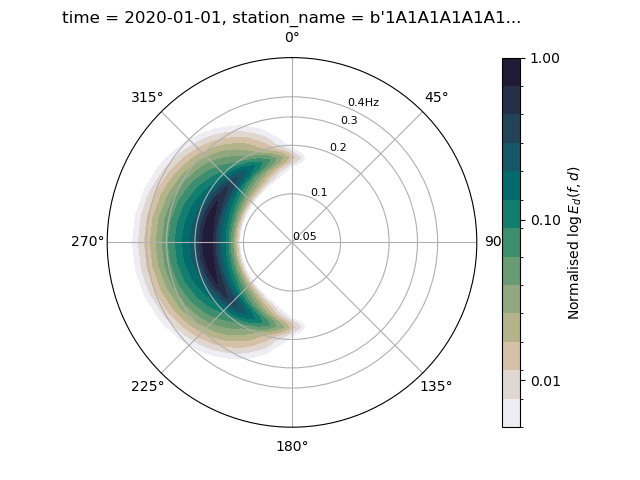
\includegraphics[width=0.8\linewidth]{Figures/figures/jonswap-wavespectra3.png}
\end{center}
\end{minipage}\begin{minipage}{0.48\textwidth}
\caption{Spectre de JONSWAP orienté à 270 degré selon la convention océanographique (les vagues se propagent de l'ouest vers l'est).}\label{fig:jonswap}
\end{minipage}
\end{center}
\end{figure}

\begin{table}[htbp]
\caption{\label{tab:org361184d}Paramètres du spectre de vagues assimilié comme conditions frontière à l'ouest du domaine.}
\centering
\begin{tabular}{lcrcl}
\hline
\hline
Description & Symbole & Valeur & Unités & Notes\\
\hline
Constante pour Goda & -- & 0.205 & ? & \Textcite{goda1988variablity}\\
\emph{Energy level of PM spectrum} & \(\alpha\) & 0.0081 & -- & \Textcite{wwiii2016user} (Constante de Phillips)\\
\emph{Peak enhancement factor} & \(\gamma\) & 3.3 & -- & \Textcite{hasselmann1973measurements,wwiii2016user}\\
\emph{Spread with GAMMA} & \(\sigma_A\) & 0.07 & -- & \Textcite{hasselmann1973measurements,wwiii2016user}\\
\emph{Spread with GAMMA} & \(\sigma_B\) & 0.09 & -- & \Textcite{hasselmann1973measurements,wwiii2016user}\\
Moyenne directionnelle & \(\theta_m\) & 90 & degrés & \Textcite{wwiii2016user} (Convention océanographique)\\
\hline
\emph{Peak frequency} & \(f_m\) & 1/6 & Hz & (Maîtrise d'Eliot Bismuth)\\
Hauteur significative des vagues & \(h_s\) & 1 & m & (Maîtrise d'Eliot Bismuth)\\
\hline
\end{tabular}
\end{table}
\subsection{(À faire) Mise en oeuvre de la grille variable (Création de l'architecture)}
\label{sec:orge0f6f58}

\textbf{Sous-mailles} : On a vu des grilles avec des mailles de 25 \(\mathrm{km}^2\). Est-ce qu'on peut se permettre de faire des sous-mailles? Je pense que c'est assez simple avec \emph{Wavewatch}, car il y a un facteur de division. Au final, il faut modifier :
\begin{itemize}
\item Le \textbf{facteur de division};
\item La \textbf{longueur du domaine};
\item La \textbf{largeur du domaine}.
\end{itemize}

Que faut-il transformer pour avoir plusieurs résolutions :
\begin{itemize}
\item[{$\boxtimes$}] Il faut qu'on ait un \textbf{dossier pour chaque résolutions individuelles}. Ainsi, on va avoir besoin d'une fonction \emph{create cases} qui permet de \emph{dispatcher} ou distribuer les dossiers tout en créant de nouvelles séries de paramètres.
\item[{$\boxtimes$}] Il faut modifier tous les \emph{build grids} car les MAPSTA vont être différentes, tout en gardant la même longueur horizontale. On a donc besoin de
\begin{itemize}
\item « \emph{nx} »  : le nombre de points dans la grille en x.
\item « \emph{sdf} » : le \emph{scaling (division) factor}.
\item « \(\Delta x\)  : la longueur horizontale des mailles.
\end{itemize}
\item[{$\boxtimes$}] Il faut modifier les \emph{boundary points}, car les coordonnées aussi vont être asses différentes, il faut que le point soit toujours situé au \emph{scaling division factor} techniquement..
\item[{$\boxtimes$}] Faudrait aussi trouver un moyen que les paramètres soient intégrés dans le cas pour avoir de l'information, donc tous les sous-routine Python doivent pouvoir être exécutées à partir du dossier courant.
\begin{itemize}
\item On peut les copier [C'est ça que j'ai du faire, même si ça implique de la redondance].
\item On peut aussi créer un lien symbolique (J'ai essayé et ça ne marche pas, car ça utilise son propre répertoire courant).
\end{itemize}
\item[{$\boxtimes$}] Faut reconstruire l'architecture des dossiers et des \emph{launchers} en langage \emph{bash} pour que tout soit harmonisé. Donc, on a maintenant un dossier \emph{cases} où l'on retrouve tous les cas individuels. On utilise seulement le \emph{work} comme endroit de départ pour copier les nouveaux fichiers lorsqu'on utilise la routine \emph{bash} « \emph{create cases} ». Cette sous-routine va aussi copier tous les paramètres nécessaires dans le module Python \emph{PARAMS.py}.
\item[{$\boxtimes$}] Finalement, il faut reconstruire le système de \emph{dispatchage} des floes (la fonction Python \emph{build ice.py}), de sorte à ce qu'on puisse controler les sous-mailles (donc la concentration de glace et les endroits où la glace se trouve).
\item[{$\square$}] Il faut aussi vérifier comment la \emph{ice concentration cutoff} a un effet sur nos \emph{runs}. Je pense que ça va nous gosser tout au long du parcours, car je ne sais pas trop comment la modifier.
\end{itemize}
\section{Résultats 1}
\label{sec:orgf14ba75}
Quelques cas intéressants\ldots{}

\begin{center}
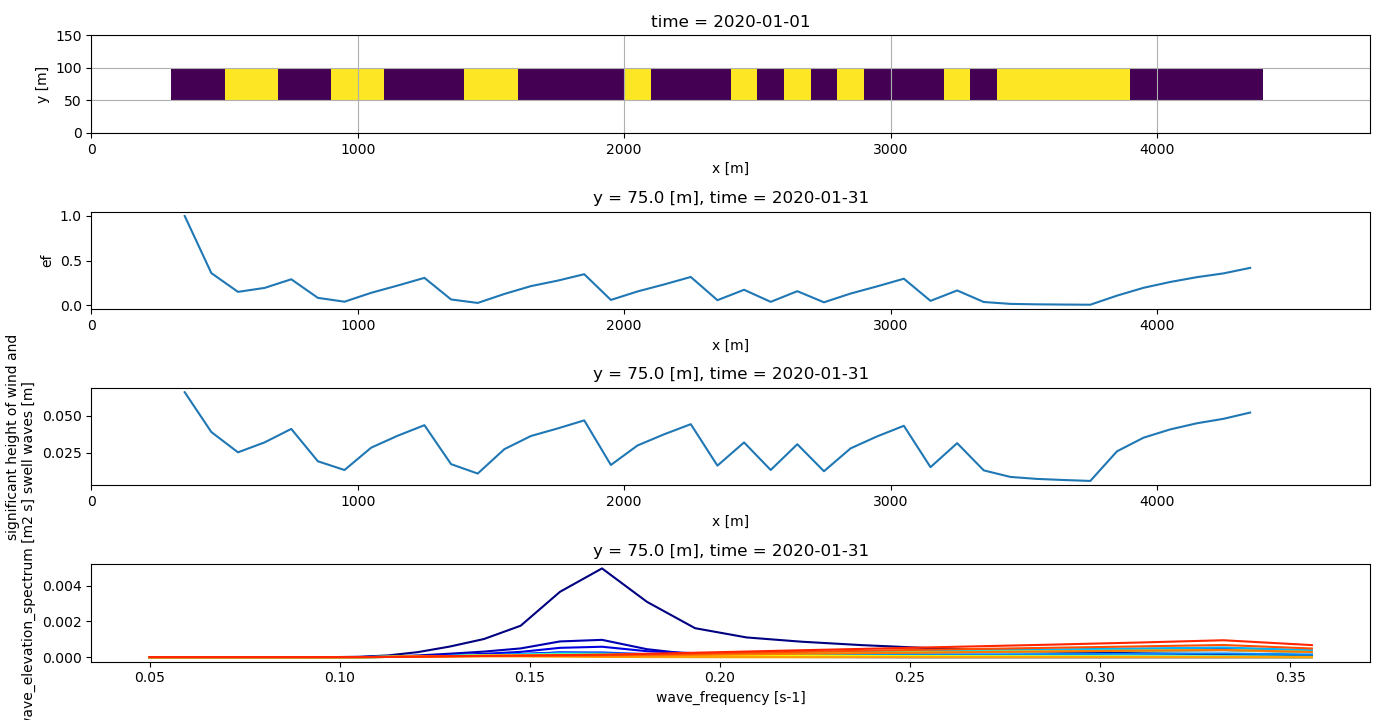
\includegraphics[width=.9\linewidth]{Figures/figures/analyse_spec_ww3_001.png}
\end{center}

Comparaison des spectres initiaux et finaux. 

\begin{center}
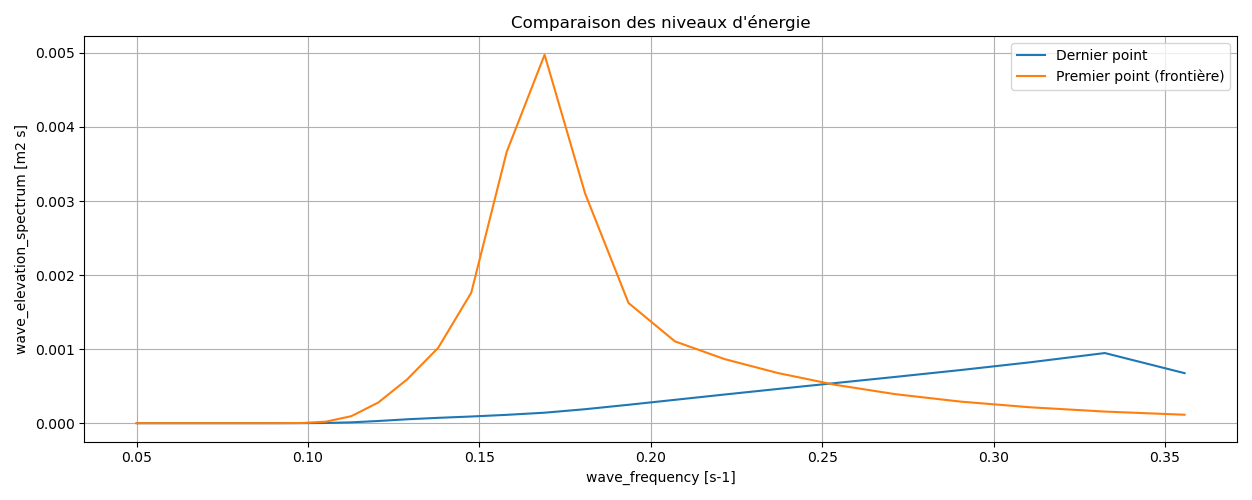
\includegraphics[width=.9\linewidth]{Figures/figures/spectre001.png}
\end{center}

Raisons du pourquoi on a ça : 
\begin{itemize}
\item Il y a un \emph{ice concentration cutoff} que je viens de trouver.
\begin{quote}
\emph{Miscellaneous (user def. values) :}

\texttt{================================================}

\emph{WAVEWATCH-III WARNING IN W3GRID :}

\emph{CICE0.NE.CICEN requires FLAGTR>2}

\emph{Parameters corrected: CICE0 = CICEN}

\emph{Ice concentration cut-offs  :    1.00  1.00}

\emph{Wind input reduction factor in presence of ice :  1.00}

\emph{(0.0==> no reduction and 1.0==> no wind input with 100\% ice cover)}

\emph{Space-time extremes DX-Y set to default 1000 m}

\emph{Space-time extremes Dt set to default 1200 s}
\end{quote}
\end{itemize}


Nos switches (En ce moment, on prend IC4 avec la \emph{ICE method 1} : 
\begin{quote}
\emph{F90 NOGRB NOPA LRB4 NC4 SHRD PR3 UQ FLX0 LN1 ST3 NL1 BT1 DB1 TR0 BS0 IC4 IS0 REF1 XX0 WNT2 WNX2 CRT2 CRX2 O0 O1 O2 O3 O5 O7 O11}
\end{quote}
Donc on a
\begin{equation}
   \alpha = \exp{\frac{-2\pi C_{ice,1}}{\sigma} - C_{ice,2}}
\end{equation}
\section{Résultats 2 : Distribution de glace (ICEM1)}
\label{sec:org6e00a00}



\begin{figure}[!h]
\begin{center}
\begin{minipage}{\linewidth}
\begin{center}
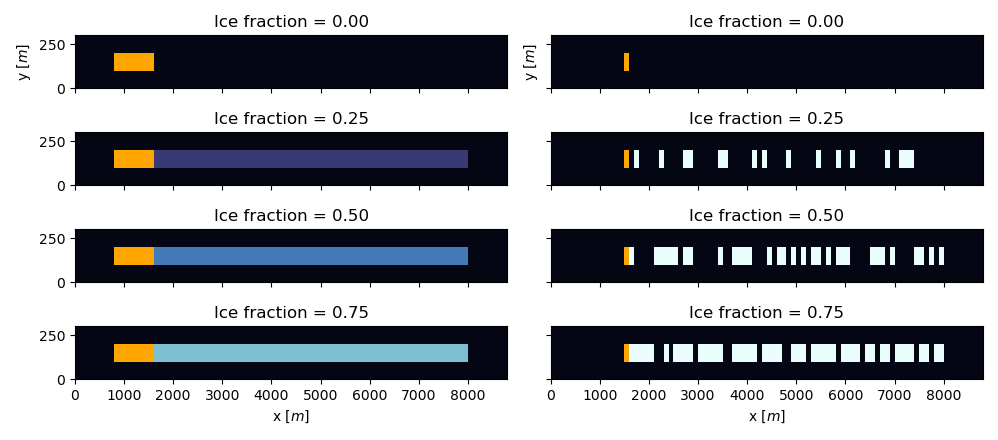
\includegraphics[width=\linewidth]{Figures/figures/ice_distributions001.png}
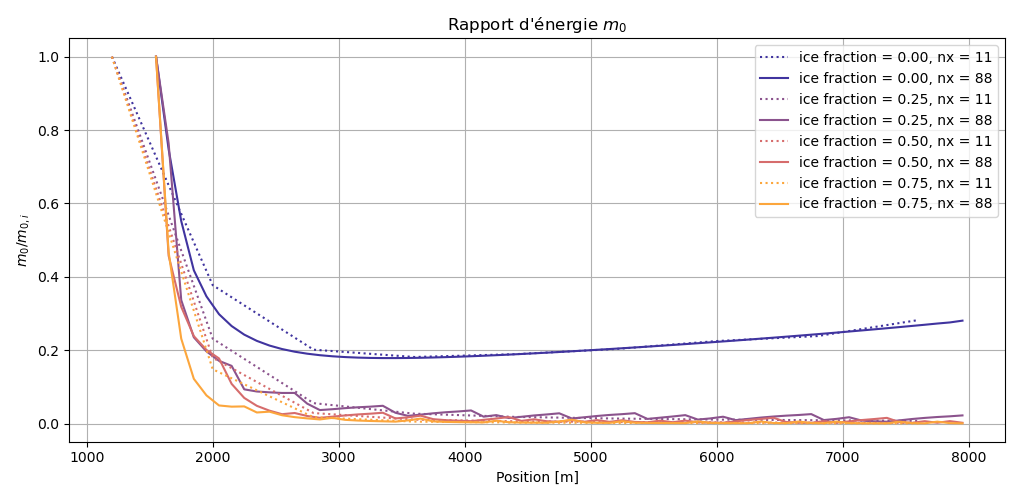
\includegraphics[width=\linewidth]{Figures/figures/analyse_spec_ww3_002.png}
\end{center}
\end{minipage}
\begin{minipage}{0.8\textwidth}
\caption{En haut, les 8 distributions de glace à l'étude. En bas, Rapport de l'énerge initiale (au point frontière) versus l'endroit sur le domaine. Autrement dit, énergie normalisée par la valeur en « \textit{input} ».}
\label{fig:jonswap}
\end{minipage}
\end{center}
\end{figure}

Et quelques spectres

\begin{center}
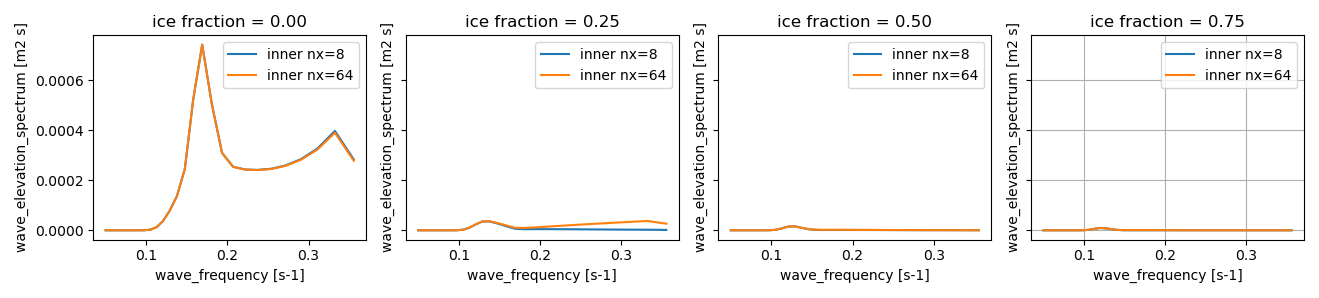
\includegraphics[width=.9\linewidth]{Figures/figures/analyse_spec_ww3_003.png}
\end{center}
\begin{center}
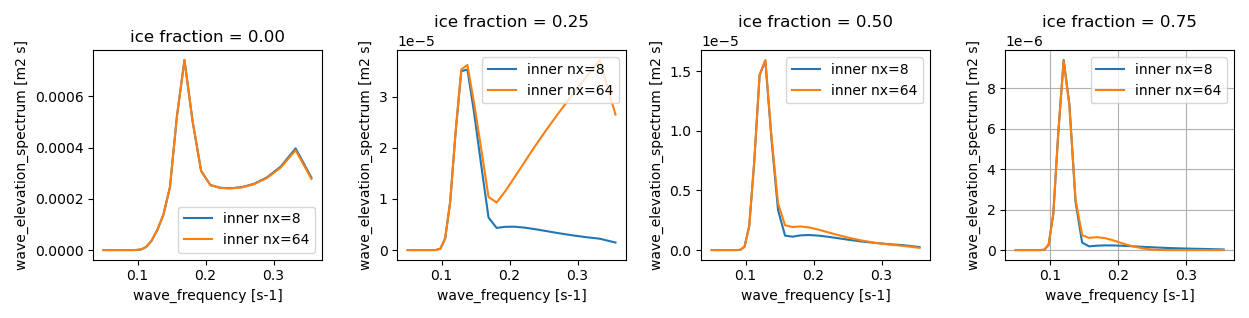
\includegraphics[width=.9\linewidth]{Figures/figures/analyse_spec_ww3_004.png}
\end{center}
\section{Généralisation du modèle en 2 dimensions}
\label{sec:org49793ad}



\tikzmath{\lx=24;\ly=6;}
\tikzmath{\lxm=20;\lym=4;}


\begin{figure}[!h]
\begin{center}
   \begin{tikzpicture}[scale=0.7]
      % MidnightBlue!25
      % BrickRed!25
      % Green!25
      \fill [color=Green!25] (0,0) rectangle (\lx,2);
      \fill [color=Green!25] (0,\ly-2) rectangle (\lx,\ly);
      \fill [color=Aquamarine!75] (4,2) rectangle (\lx-4,4);
      \fill [color=BrickRed!35] (7,2) rectangle (8,4);
      \fill [Dandelion!35] (20,2) rectangle (24,4);
      \fill [Dandelion!35] (0,2) rectangle (7,4);
      % Lignes blanches : 
      \foreach \y in {0,...,\ly} {
         \draw [ultra thick, white] (0,\y) -- (\lx,\y);
         \foreach \x in {0,1,...,\lx} {
            \draw [ultra thick, white] (\x,0) -- (\x,\ly);
            }
         }
      % Grille lignée
      \foreach \y in {2,4,...,\lym} {
         \draw [ultra thin, gray] (0,\y) -- (\lx,\y);
         \foreach \x in {4,8,...,\lxm} {
            \draw [ultra thin, black] (\x,0) -- (\x,\ly);
            }
         }
      % Annotations : 
      \draw [black] (0,0) rectangle (\lx,\ly);
      \draw [black,|{latex}-{latex}|] (8,-0.5) -- (14,-.5) node[fill=white] {$(n_{x,0}-3)\times2^k = 4\times 2^n$} --(20,-0.5);
      \draw [black,|{latex}-{latex}|] (0,7) -- (12,7) node[fill=white] {$n_{x,0}=6$} --(24,7);
      \draw [black,|{latex}-{latex}|] (0,7) -- (12,7) node[fill=white] {$n_x=24$} --(24,7);
      %\draw ;
      \draw (22,1.5) node [] {$nx=24$};
      % Légende
      \draw [thin] (7,-1.8) rectangle (17,-4);
      \filldraw[Green!25] (8,-2) rectangle (8.8,-2.8);
      \draw (9,-2.4) node [right] {Terre};
      \filldraw[Aquamarine!75] (8,-3) rectangle (8.8,-3.8);
      \draw (9,-3.4) node [right] {Mer};
      \filldraw[BrickRed!25]  (12,-2) rectangle (12.8,-2.8);
      \draw (13,-2.4) node [right] {Points frontière};
      \filldraw[Dandelion!35]  (12,-3) rectangle (12.8,-3.8);
      \draw (13,-3.4) node [right] {Non-définit};
   \end{tikzpicture}
   \begin{minipage}{0.8\linewidth}
   \end{minipage}
\end{center}
\caption{\label{org69def4b}Schématisation de la grille sous-jacente du modèle lors de la généralisation en 3 dimentions.}
\end{figure}


Pour que tous nos modèles puissent fonctionner en deux dimensions, il faut absolument ajouter un \emph{sdf} (\emph{scaling division factor}) en \emph{x} et un \emph{sdf} en \emph{y}. C'est ce qui nous permet de diviser les cases en plus petites sections individuelles (les sous-mailles), de sorte à pouvoir évaluer l'effet de la résolution sur le modèle, comme on peut l'observer à la figure \ref{org69def4b}. \medskip

\textbf{Modification nécessaires} pour passer en 2 dimensions : 
\begin{itemize}
\item[{$\boxtimes$}] \emph{ww3 grid.inp} ;
\begin{itemize}
\item La grille doit abolument sortir en 2 dimensions, de sorte qu'on puisse avoir un mur de points frontière à l'ouest.
\item Le résultat serait la \emph{mapsta} qu'on obtient à la figure \ref{org69def4b}.
\end{itemize}
\item[{$\boxtimes$}] \emph{PARAMS EMPTY.py} ;
\begin{itemize}
\item C'est notre fichier central de paramètres. C'est à cet endroit que toutes nos fonctions en Python doivent utiliser pour créer les grilles, etc.
\end{itemize}
\item[{$\boxtimes$}] \emph{create cases.sh} ;
\begin{itemize}
\item La routine \emph{bash} dans le dossier \emph{cases} qui doit créer toutes les \emph{runs} nécessaire avec toutes les longueurs physique et paramètres nécessaire.
\item Cette routine vient justement modifier toutes les autres, comme \emph{PARAMS} par exemple.
\end{itemize}
\item[{$\boxtimes$}] \emph{build grid.py} ;
\begin{itemize}
\item On doit s'assurer que la fonction \emph{create cases.sh} vienne bien modifier ce fichier Python d'\emph{inputs}.
\item C'est ici qu'on crée la grille pour Wavewatch III, donc on mentionne le \(\Delta x\), le \emph{nx} et la largeur du domaine \(L_x\) et \(L_y\), puis finalement la position du premier point dans le quadrant x-y.
\end{itemize}
\item[{$\boxtimes$}] \emph{build ice.py} ;
\begin{itemize}
\item Crée nos cartes de glace. On passe de 1D à 2D.
\item Pour l'instant on a trois quantités produites par cette routine Python, soit la \emph{ice fraction} (\(f_i\)),la \emph{ice thickness} (\(h\)) et le diamètre moyen des floes, soit \(\expval{D}\).
\end{itemize}
\item[{$\boxtimes$}] \emph{build spectrum.py} ;
\begin{itemize}
\item[{$\boxtimes$}] Il faut que ça crée un nombre \emph{sdfy} de points frontière, donc la création de multiples fichiers NetCDF de \emph{boundary points} ;
\item[{$\boxtimes$}] Il faut aussi que la position de ces fichiers NetCDF soit précise de manière à être générale avec les deux dimensions du domaine, donc il va falloir que ça prenne des informations variables du module \emph{PARAMS.py}.
\end{itemize}
\item[{$\boxtimes$}] \emph{ww3 bounc.inp} : Il faut s'assurer que la sous-routine Python \emph{ww3 bounc} puisse bien incorporer tous nos fichiers de spectre pour les points frontière.
\begin{itemize}
\item[{$\boxtimes$}] Donc, il faut aussi que la routine \emph{bash} \emph{create cases.sh} puisse rajouter des fichiers dans le fichier d'\emph{input} \emph{ww3 bounc.inp} du même coup. Alors, il faut trouver un moyen de padder du texte dans tout ça.
\end{itemize}
\end{itemize}
\subsection{À faire lorsque le modèle est set-up en 2D}
\label{sec:org9b4a561}
\begin{itemize}
\item[{$\boxtimes$}] Vérifier que les résultats sont semblables pour 2 résolutions différentes.
\begin{itemize}
\item On refait cette expérience avec un ligne.
\end{itemize}
\item[{$\boxtimes$}] Intégrer le vent dans la routine \emph{create cases.sh}, de sorte à ce qu'on puisse regénérer une figure comme Éliot Bismuth.
\begin{itemize}
\item La figure, c'est la concentration de glace vs la force du vent.
\end{itemize}
\item[{$\square$}] Finalement, vérifier que les expériences sont les mêmes pour une plus grande résolution en 2 dimensions.
\end{itemize}


\printbibliography
\end{document}
